\chapter{UCNA Analysis}
\label{ch:UCNA_Analysis}
%%%%%%%%%%%%%%%%%%%%%%%%%%%%%%%%%%%%%%%%%%%%%%%%%%%%%%%%%%%%%%%%%%%%%%%%%%%%%%%
%%%%%%%%%%%%%%%%%%%%%%%%%%%%%%%%%%%%%%%%%%%%%%%%%%%%%%%%%%%%%%%%%%%%%%%%%%%%%%%
%%%%%%%%%%%%%%%%%%%%%%%%%%%%%%%%%%%%%%%%%%%%%%%%%%%%%%%%%%%%%%%%%%%%%%%%%%%%%%%

\iffalse
Designing an experiment and collecting the right data are non-trivial alone,
but interpreting the results lends itself to a whole new train of thought.
The rest of this thesis is spent describing the details of such an
analysis, with this chapter summarizing important aspects,
such as terminology to be used later and the
model used to characterize our detector response.
\fi

This chapter is dedicated to introducing important aspects of the analysis that
is not strictly tied to calibrations and asymmetry extraction, but rather
data collection and processing to turn raw detector signals into values that
can be calibrated and analyzed. 

\section{Data Taking Structure}

The data is broken into three types of run periods, namely $\beta$-decay data, source calibration, and
Xe position mappping. The latter two determine the parameters of the energy calibration to be
applied to the data runs. The source calibration and Xe position mapping run periods
occur periodically throughout each data set and are applied to surrounding $\beta$-decay runs. This
creates different subsets of data to which each calibration is applied, as will be illustrated
throughout the rest of this dissertation. Here we simply highlight the structure of the
$\beta$-decay runs, and one should take note that the source calibrations and Xe position map periods
are spaced throughout.

\subsection{$\beta$-decay run structure}
We utilize what we call an octet run structure, where each octet contains a total of twenty-four
runs, eight of which are $\beta$-decay data runs, eight of which are background runs, and eight
of which are depolarization runs. The octet is further split into two halves, A and B, which define
the order of the runs within them as seen in table \ref{tab:octetStructure}. Whether the A structure
or the B structure comes first within an octet is determined randomly. There are four $\beta$-decay
runs of each spin-state (aligned and anti-aligned to the magnetic field in the spectrometer), and their
accompanying background runs allow for background subtraction. 

\begin{table}[h]
  \caption{Octet structure, where $\pm$ indicates spin flipper on/off,
    B refers to background run, D refers to depolarization run, and $\beta$
    refers to $\beta$-decay runs.} 
  \centering
  \begin{tabular}{llllllllllll}
    \hline \hline \\ [-1.75ex]
    A1 & A2 & A3 & A4 & A5 & A6 & A7 & A8 & A9 & A10 & A11 & A12 \\ 
    B$^-$ & $\beta^-$ & D$^-$ & B$^+$ & $\beta^+$ & D$^+$ & $\beta^+$ & D$^+$ & B$^+$ & $\beta^-$ & D$^-$ & B$^-$ \\
    \hline \\ [-1.75ex]
    B1 & B2 & B3 & B4 & B5 & B6 & B7 & B8 & B9 & B10 & B11 & B12 \\
    B$^+$ & $\beta^+$ & D$^+$ & B$^-$ & $\beta^-$ & D$^-$ & $\beta^-$ & D$^-$ & B$^-$ & $\beta^+$ & D$^+$ & B$^+$ \\
    \hline
  \end{tabular}
  \label{tab:octetStructure}
\end{table}



\section{Backscattering} \label{sec:backscattering}
Before moving forward, it is important to formally introduce the different
backscattering events, as they will be referenced often. A backscattering
event is an electron event initially emitted towards one detector, but that
is scattered through a large enough angle that its momentum is reversed and
it travels to the opposite detector. Some of these events are backscattered
by a detector component and can therefore be identified as having backscattered
due to energy deposition on both sides,
while others backscatter without depositing enough energy (or backscatter prior
to reaching the detector) and therefore become what we call ``missed''
backscattering events. Missed backscattering events are problematic as they
are assigned the wrong intitial direction and therefore systematically effect
the asymmetry.

\begin{figure}[h]
\centering
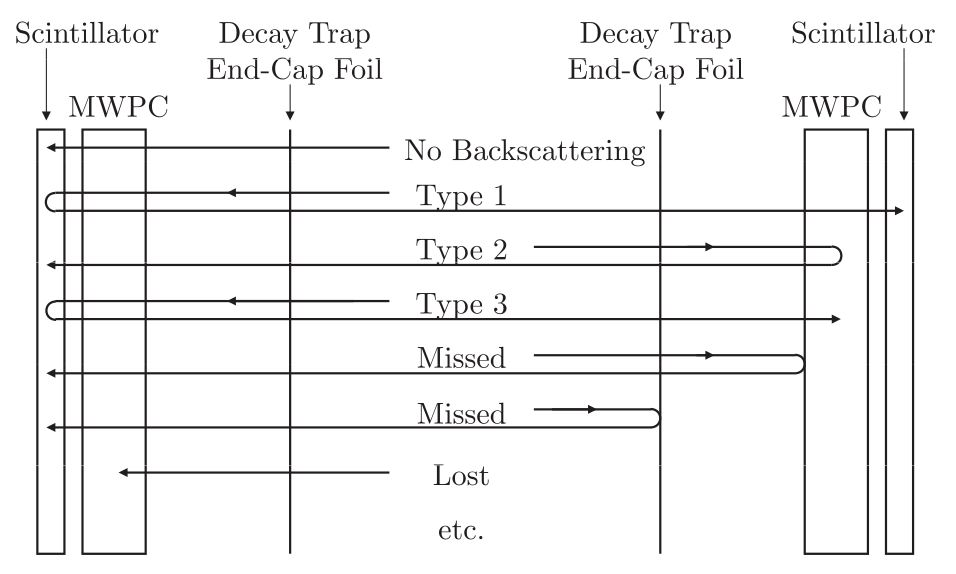
\includegraphics[scale=.4]{3-UCNAAnalysis/backscatterSchematic.png}
\caption{Schematic of different event types and the trigger logic involved with identifying
  each type \cite{plaster2012}.}
\label{fig:backscatterSchematic}
\end{figure}

Based on which detector components trigger, we classify events
into those that do not backscatter
(Type 0) and those that do backscatter (Types 1, 2, and 3) \cite{plaster2012}.
A schematic of the different event types can be seen in figure \ref{backscatterSchematic}.
Type 0 events
trigger one scintillator and one MWPC on the same side, while Type 1 events trigger
both scintillators and both MWPCs. For such events, we assign the initial
direction to the triggering detector for Type 0 and to the earlier triggering detector
for Type 1. Type 2/3 events comprise a class of events that backscatter and trigger both
MWPCs, but only trigger a single scintillator.
The initial direction of such events can
not be determined from trigger logic alone, as can be demonstrated by considering two events
which look identical under trigger logic.
For example, let ``Event 1'' denote an event that initially backscatters off
of MWPC 1 before reaching scintillator 1
and then traverses the length of the decay
trap to trigger both MWPC 2 and scintillator 2 on the opposite side.
Then, suppose ``Event 2'' denotes another event emitted
in the opposite direction to event 1. Suppose this event
triggers MWPC 2 and scintillator 2
only to backscatter from the scintillator and travel to MWPC 1 and stop short
of scintillator 1. Both events trigger MWPC 1 and 2 and scintillator 2,
but the two events had opposite initial directions, so inclusion of the
two events without further knowledge of their initial direction creates
a dilution to the asymmetry.

An important distinction, however, does exist between Type 2 and Type 3 events:
Type 2 events only pass through the MWPC on the
triggering scintillator side once, whereas Type 3 events scatter from
the scintillator, and therefore pass through the MWPC twice on
the triggering side. We can consequently apply a cut on the energy deposited in
the MWPC on the triggering side to statistically assign
Type 2/3 events to the correct side.
This drastically reduces
Monte Carlo corrections for such backscattering events as simulation indicates we
properly identify $>80\%$ of all Type 2/3 events across all energies using this
technique, a marked
improvement over the roughly $50\%$ misidentification rate without separation.





%--------------------------------------------------------------

\section{Outline of Analysis Steps}

To preface the rest of this chapter, we can highlight
the general process of the analysis beginning with a raw detector
ADC value from each PMT and finishing with an asymmetry.
Below are the general steps:

\begin{itemize}
\item Determine pedestals for each PMT and subtract the pedestal from each data event.
\item Measure the gain of each PMT and divide the drifts out of the signal.
\item Apply a PMT-by-PMT calibration to determine the expected position dependent
  energy deposited in the scintillator
  for each event.
\item Correct for the position dependent response of each PMT
  to return a visible energy as seen by each PMT, $E_{\mathrm{vis},i}$.
\item Combine the four PMT energies into a single deposited energy, $E_{\mathrm{vis}}$.
\item Convert this combined estimate of the energy deposition to a final
  reconstructed energy, $E_{\mathrm{recon}}$, to use in analysis.
\item Calculate an asymmetry and apply all systematic corrections.
\end{itemize}

It is important to point out early on the difference between $E_{\mathrm{vis}}$ and
$E_{\mathrm{recon}}$. The deposited or visible energy, $E_{\mathrm{vis}}$, is the energy
physically deposited in the
scintillator by a particle, while the reconstructed energy, $E_{\mathrm{recon}}$, is an estimate of
the true initial energy of an event. The two are different due to the electron losing energy
as it traverses through the windows of the decay trap, the windows of the MWPC,
the MWPC itself, and the dead layer of the scintillator. Of course the analysis could be
done in terms of $E_{\mathrm{vis}}$, but it is more convenient to express the results
in terms of the true electron energy spectrum, and also the energy dependent theory modifications
are in terms of the true initial energy of an event.


\section{Energy Response from Detector Response} \label{sec:EnergyResponse}
Following the process outlined in the previous section, we can derive an
expression which takes a detector signal to an energy estimate for each PMT.
The visible energy $E_{\mathrm{vis},i}$ deposited
in the scintillator as seen by a single PMT $i$ for an event at position $(x,y)$ 
is given by the following: 

\begin{equation} \label{eq:EvisResponse}
E_{\mathrm{vis},i} = \eta_i^{-1}(x,y) \cdot f_i\Big[ \Big( \mathrm{ADC}_i - p_i(t) \Big) \cdot g_i(t) \Big]  ,
\end{equation}

\noindent where 
\begin{align*}
&f_i = \textrm{linearity relation from ADC channels to Energy,}\\
&\eta_i(x,y) = \textrm{PMT correction factor for position dependence,} \\
&p(t) = \textrm{mean pedestal value for PMT } i,\\
&g(t) = \textrm{gain correction factor for PMT }i.
\end{align*}

This expression is exact in the case where all values are determined with infinite
precision and without stochastic fluctuations. Unfortunately, each parameter on the right
side of this equation is either stochastic in itself (as is the ADC response), or it was
determined via observation of a stochastic process (the gain and pedestal), and so
the underlying value for any given event may not be the same as the value applied in the
above expression. Thus what we
really resolve is an approximation to the energy, which comes with some uncertainty. This
uncertainty will be addressed later in section \ref{ssec:energyRecon}.
For the time being, keep in mind the above list of
input parameters which take us from an ADC signal (detector signal) to an energy signal. 

\subsection{Combining PMT Responses}

\subsection{$E_{\mathrm{vis}}$ to $E_{\mathrm{recon}}$}



\section{Time-dependent Detector Corrections}

Obviously the system is not immune to drifts in signals due to variations
in time. There are many sources of such drifts, ranging from simple
electronic noise to changes in temperature. We deal with such time-dependent
effects using pedestal subtraction, gain correction, and constant monitoring
of backgrounds.

\subsection{Pedestal Subtraction}
The pedestal is a measure of the inherent detector signal, or baseline, 
upon which all other data signals lie. In terms of PMT signals, you can imagine 
the pedestal as a non-zero ADC value corresponding to zero input, or an offset.
You might say that the experiment can be run without caring about an offset
because the calibration will take this into account, which would be the case 
if the pedestals were constant or if we calibrated each run against itself, but 
neither is the case. We use a collection of subsequent runs to form our 
calibration sets, and these sets then calibrate data which is often taken hours,
or even days, earlier or later. Thus changing pedestals can be worrisome, and care
must be taken to determine the pedestals and subtract them from data.

To determine a pedestal, events must be chosen where there was a global trigger, but
the PMT of interest does not trigger and preferably there is no signal
whatsoever in the scintillator on that side. Obvious choices for these events are
UCN monitor triggers, opposite side two-fold PMT triggers, and high-threshold $^{207}\mathrm{Bi}$
pulser triggers from other PMTs. Once there is a global trigger, we can use the individual TDC
to ensure there was no individual trigger, and the events can be 
histogrammed for the PMT of interest. This leads to pedestals like those seen in
figure \ref{fig:peds_ind}. The mean of this peak can be taken as the average pedestal for a single run,
and this value can be 
subtracted from every subsequent reading of this PMT.

One interesting thing to note is that the discriminators, which determine whether
a component triggers,
for all PMTs are housed 
together, which leads to correlations between the PMT triggers. In a perfect world, 
each PMT would have one pedestal, and that pedestal wouldn't care about other PMT's signals.
Instead, what we see in figure \ref{fig:peds_types} is that the pedestals
can be dependent on the type of events that are chosen 
to construct the pedestal. This indicates that the pedestal for one PMT may be dependent
on the signal present in another PMT. These shifts are important as a
pedestal shift of ~5-10 channels maps to an offset of roughly
~5-10 keV, as the PMTs show roughly 1:1 correspondence between ADC and keV.

The influence of event type on pedestal values means we must carefully choose which events
to use when calculating the pedestal.
The best choice would be UCN monitor events due to there being zero signal 
in the electronics box housing the PMT electronics, and these thus would give
the cleanest measurement of the PMT pedestal.
These are unfortunately the first event type we can eliminate as they are only present
during $\beta$-decay runs (when UCN are produced and thus create UCN monitor triggers)
and not during calibration runs (taken during the day when the beam is off). 
Of the remaining two options, the choice was made to use the
two-fold PMT triggers from the opposite detector rather than $^{207}\mathrm{Bi}$ pulser
events. The choice is somewhat arbitrary, because what is important is that we choose
a consistent subset of data for both calibration and $\beta$-decay data, but the
opposite side two-fold triggers do better represent the baseline present in each PMT
for data events when compared to the much higher signal present from the $^{207}\mathrm{Bi}$
pulser.


\begin{figure}[h] 
\centering

\includegraphics[scale=.25]{3-UCNAAnalysis/ImageHolder.pdf}
\caption{Pedestal values for a $\beta$-decay run determined using different 
types of events to illustrate the cross-talk between PMTs. (UCN Monitors, 
Bi triggers, Opposite side triggers, same side 2-fold triggers. Also shown 
is the dependence of the pedestal on which PMT triggers in the Bi Pulser. NOTE:
Choose West PMT4 in an early 2012/2013 beta run) }
\label{fig:peds_types}
\end{figure}

\begin{figure}[h] 
\centering

\includegraphics[scale=.25]{3-UCNAAnalysis/ImageHolder.pdf}
\caption{Example pedestals from all 8 PMTs}
\label{fig:peds_ind}
\end{figure}

With the event type chosen, we extract the mean and RMS of the pedestal peak (see figure
\ref{fig:peds_ind}) for each PMT in every run. The pedestal mean (referred to as simply
the pedestal) is then subtracted from the ADC values for all events. This effectively
removes the time-dependent baseline from the detector signals. The time dependence of
the pedestals can be seen for the East PMTs from 2011-2012 in figure \ref{fig:peds_timeDep}.
Most of the PMTs have pedestals which remain quite stable, but PMT East 3 shows the
importance of a run-by-run pedestal subtraction.

\begin{figure}[p]
\centering
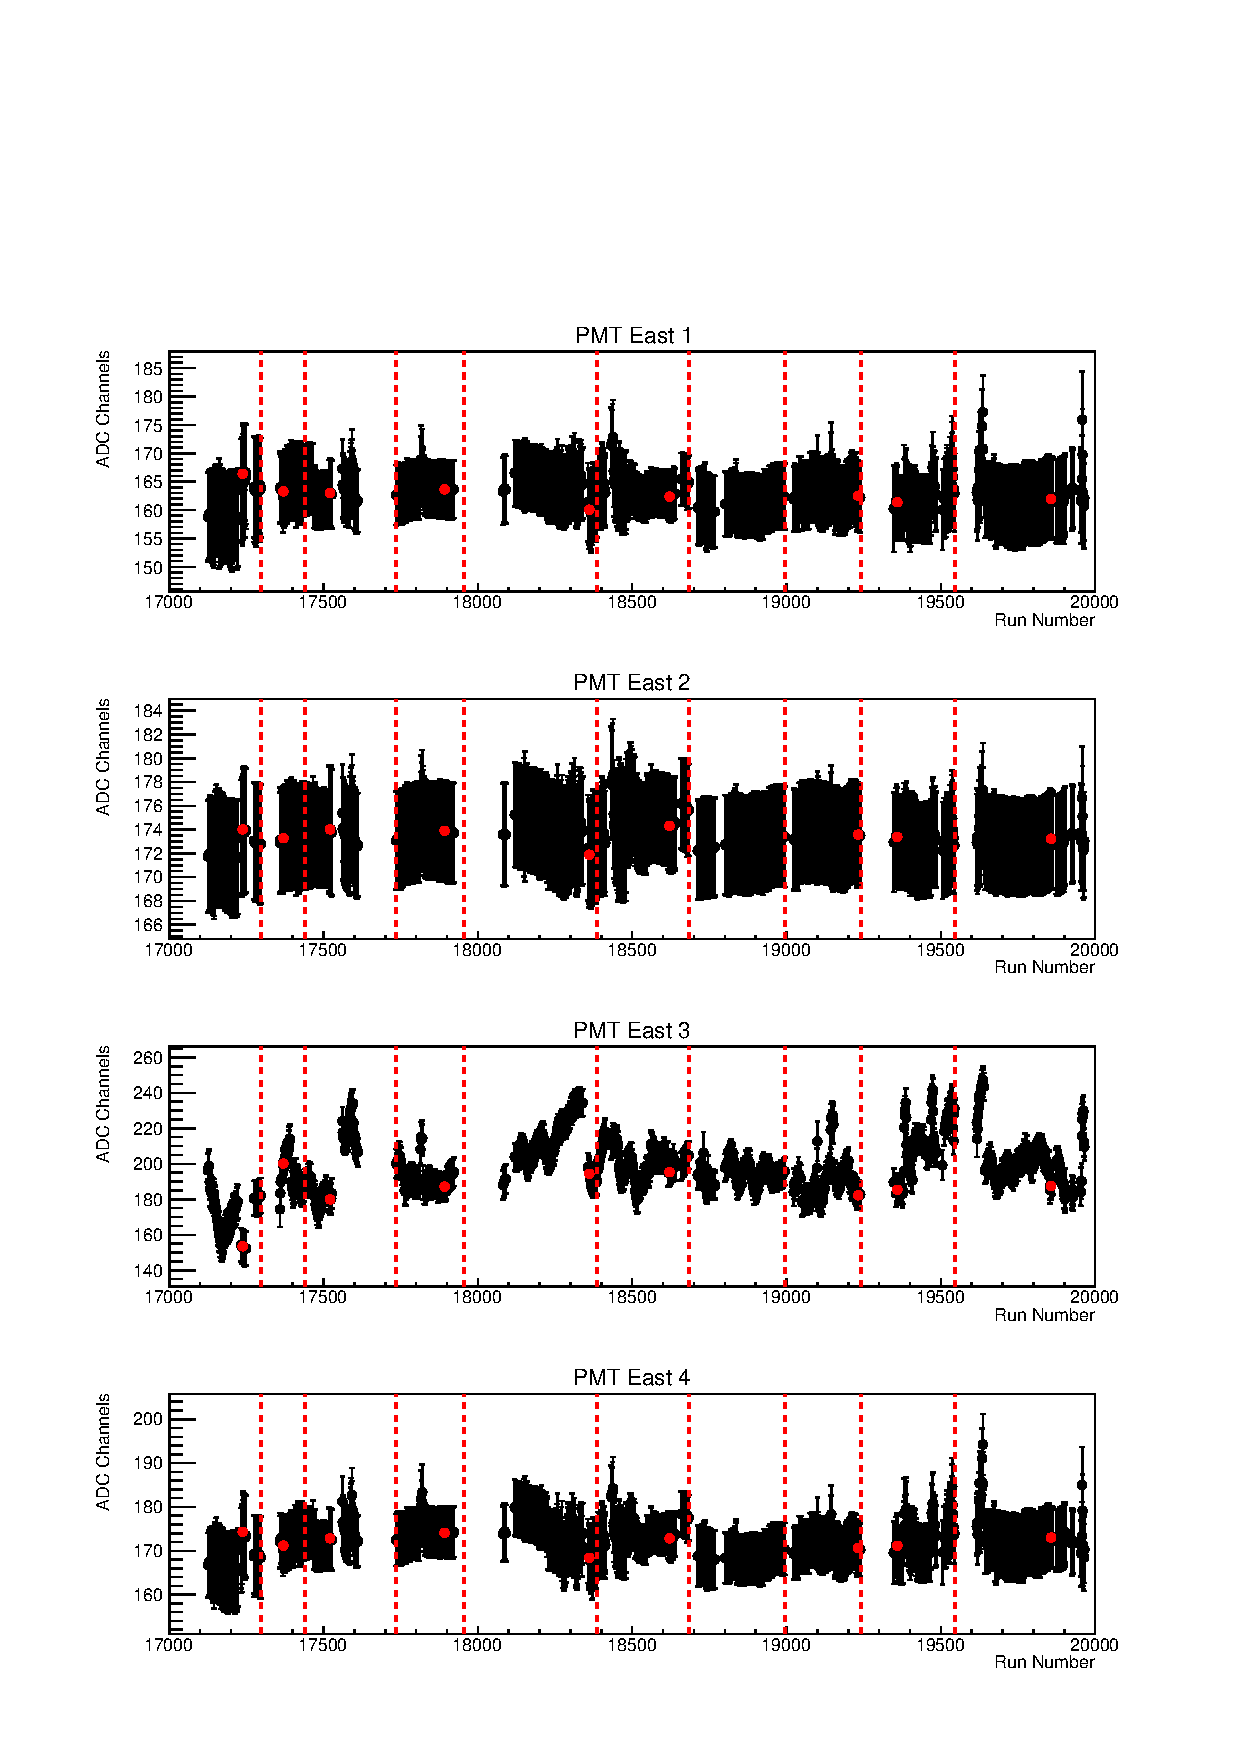
\includegraphics[page=1,scale=0.8]{3-UCNAAnalysis/2011-2012_pedestals.pdf}
\caption{Pedestal means as a function of run number for 2011-2012 East Detectors. Error bars are the
  RMS of the measured pedestal. The red lines indicate what ranges of runs belong to
  different calibration periods, and the red marker is the calibration reference run,
  which will be discussed in later sections.}
 \label{fig:peds_timeDep}
\end{figure}

\begin{figure}[p] 
\centering
\includegraphics[page=2,scale=0.8]{3-UCNAAnalysis/2011-2012_pedestals.pdf}
\caption{Pedestal means as a function of run number for 2011-2012 West Detectors. Error bars are the
  RMS of the measured pedestal. The red lines indicate what ranges of runs belong to
  different calibration periods, and the red marker is the calibration reference run,
  which will be discussed in later sections.}
\label{fig:peds_timeDep}
\end{figure}

\subsection{Gain Correction}

\subsubsection{$^{207}\mathrm{Bi}$ Pulser}
%The goal of the $^{207}\mathrm{Bi}$ gain monitoring pulser system is to create a standard
%candle type signal present in all PMTs to be tracked over time. 
The primary gain monitoring system consists of a small amount $^{207}\mathrm{Bi}$
deposited within a small block of scintillator. The scintillator was surrounded by
light reflecting material on three sides, with the fourth side covered with an optical
attenuator to attempt to match the light output of the \~1~MeV conversion line in the $^{207}\mathrm{Bi}$
to the light output of 1~MeV of energy deposited in the detector scintillator. The pulser was then
attached directly to the PMT next to where the light guides attached to the PMT.
To allow for a single-PMT high threshold trigger, the signal was split off to a different
discriminator than the one used when determining a two-fold trigger. These high threshold
discriminators then allowed for pulser triggers with a distinct pulser identification \cite{mpmThesis}.

An unfortunate but low impact issue with the pulser involves the amount of attenuation applied to the
pulser signal. The pulser peak lies well beyond the equivalent of 1~MeV of light as would be produced
in the detector scintillator, and therefore far outside the range of the $\beta$-decay spectrum. This
is not a serious issue as the PMTs seem to be quite linear, so even a peak well outside the
energy range of interest should suffice.

\begin{figure}[h] 
\centering

\includegraphics[scale=.25]{3-UCNAAnalysis/ImageHolder.pdf}
\caption{Example pedestals from all 8 PMTs}
\label{fig:biPulser}
\end{figure}

The $^{207}\mathrm{Bi}$ pulser peak is fit on a run-by-run basis, allowing for gain corrections on the time
scale of a single run. The fit was done iteratively, with the initial guesses for mean and fit range determined
by stepping backwards from the last bin and using a self-written algorithm to search for the peak. Then the the peak
was fit five times consecutively, with each successive fit being fed the previous fit's mean and sigma. This
made sure the fit converged as best as possible on the mean of the pulser peak. An example pulser peak and fit
can be seen in figure \ref{fig:biPulser}.

The method for applying the gain correction is as follows. First, a reference gain must be determined
to normalize all other gains against. This was chosen to be what is called the ``reference run'', and it
typically consists of a manually inspected source run within each source calibration period. The gain factor
is then calculated as the ratio of the pulser peak in a given run divided by the pulser peak in the reference
run, or
%
\begin{equation}
  g_i = \frac{\mu_i}{\mu_{\mathrm{ref}}}
\end{equation}
%
This automatically defines the gain of the reference run to be $g_{\mathrm{ref}}=1$. Then all other runs which are
calibrated by a certain run period have gain factors which vary based on the fitted pulser value. The time
dependence of the gain values in 2011-2012 can be seen in figures \ref{fig:2011-2012pulser_East}
and \ref{fig:2011-2012pulser_West}. The behavior is similar in 2012-2013.

Some problems with the $^{207}\mathrm{Bi}$ pulser did occur. There were several periods where the pulser
simply did not work for a certain PMT. This was always limited to a single PMT not working, and when this
was the case the PMT without a pulser signal was not used when reconstructing the energy. This has
minimal effect on the energy reconstruction though, as the ``bad'' PMT is still used when determining
a two-fold trigger, and the remaining three PMTs contain sufficient information for reconstructing the
energy deposited. Periods where $^{207}\mathrm{Bi}$ pulser information is missing are evident in
figures \ref{fig:2011-2012pulser_West} where there is missing data for certain PMTs over extended ranges.
It should be noted that in 2012-2013, West PMT4 never had a functioning pulser.

\begin{figure}[p] 
  \centering
  \includegraphics[page=3,scale=.8]{3-UCNAAnalysis/2011-2012_gain.pdf}
  \caption{Gain factors, $g_i$, as a function of run number for 2011-2012 East Detectors.
    The red lines indicate what ranges of runs belong to
    different calibration periods, and the red marker is the calibration reference run.}
  \label{fig:2011-2012pulser_East}
\end{figure}

\begin{figure}[p] 
  \centering
  \includegraphics[page=4,scale=.8]{3-UCNAAnalysis/2011-2012_gain.pdf}
  \caption{Gain factors, $g_i$, as a function of run number for 2011-2012 West Detectors.
    The red lines indicate what ranges of runs belong to
    different calibration periods, and the red marker is the calibration reference run.}
  \label{fig:2011-2012pulser_West}
\end{figure}

\subsubsection{Endpoint Stabilization}

There are unexplained longer term gain fluctuations that do not seem to be captured by the
$^{207}\mathrm{Bi}$ gain monitoring system that can be seen by monitoring the endpoint of the
$\beta$-decay spectrum. These are corrected by fitting the endpoint using a Kurie plot for each
PMT and comparing to the expected endpoint from simulation. Then a secondary gain correction
factor can be applied to match the endpoint of each PMT to the expected endpoint. The endpoints
before and after such a correction can be seen in figure \ref{fig:endpoints}, where the
large deviation over runs xxx-xxx was corrected.



\subsection{Time-dependent backgrounds}
Background events which may have some time dependence are removed from the analysis
via dedicated background runs that accompany every $\beta$-decay run.
Subtracting these background rates from the data rates accounts for backgrounds
with roughly a one hour time variation.
Any backgrounds that vary at the sub one hour level may go unnoticed, but
with a signal to background better than 50:1 the contribution from such is minimal.
The background run scheme will be addressed later in this chapter, with the background
subtraction addressed in chapter 5. 

%----------------------------------------------------

\section{Position Dependence}

\subsection{Activated Xenon}


\subsection{Position Maps}

%----------------------------------------------------------

\section{Trigger Thresholds}
An integral piece of the PMT Response Model from section \ref{sssec:pmtModel} 
is the sampling of the threshold functions to determine whether or not a detector
triggered. I'll repeat here that a 2-fold PMT trigger from one of the two electron
detectors is required to create a global electron trigger from the DAQ. In simulation
we only see the energy deposition as a whole from an individual scintillator, and then
we model the four-pmt response for that side. At low energies, this response is 
intimately entwined with the trigger threshold.

\subsection{General Model for Trigger Determination} \label{ssec:genTrigModel}
Obviously one must rely on data to determine the trigger thresholds of a detector, since
the non-step-functional shape is directly related to the stochastic nature 
of the detector and electronics. If we knew with infinite precision and 
accuracy the signal produced in a detector
and could read out the response in real time with infinite precision, 
there wouldn't be muchneed for a model to estimate trigger probabilities. 
Instead, to understand the trigger threshold, a functional 
form for the probability of a trigger need be determined using real data which may or 
may not have created a trigger in a detector/PMT. 

The most important part of determining the trigger threshold shape for 
any detector is the availability of data which was collected no matter if 
the detector or component (PMT) produced a trigger. If such a subset of 
data is available and plentiful, it is straightforward to estimate
the trigger probability by binning the data in some unit proportional to 
energy (whether in energy or something like it isn't important) and taking 
the bin-by-bin ratio of those events that triggered to all of the events in the 
sample. Plotting these ratios as a function of whatever metric was chosen tells 
you how probable an event of some value is to create a trigger.
Once you have mapped this probability, you can then sample these curves within 
simulation to apply your true trigger threshold to simulated data.

The not-so transparent part of the trigger probability comes when calculating the error of the estimate in each bin, since the numerator and denominator in the ratio are correlated. But as demonstrated in \cite{casadei2009efficiency}, the ROOT analysis framework handles efficiency errors effectively via use of Bayesian Statistics. 

PUT IN DISCUSSION OF BAYESIAN STATISTICS FOR EACH BIN AND ASYMMETRIC ERROR BARS
AND CONFIDENCE LIMITS.

\subsection{Trigger Data Selection}
As mentioned before, the data used for constructing trigger thresholds must not be 
biased towards triggering the PMT of interest. Thus that PMT must not be a mandatory 
component of the global trigger for that event, so care must be taken to choose only 
events which would trigger regardless of the behavior of the PMT of interest. One
other stipulation placed on these events is that they have an opportunity to 
deposit energy in a particular scintillator. The best choice of events which 
satisfy these conditions are those which have a two-fold trigger on the opposite side 
and then backscatter and those which trigger at least three PMTs on the side of 
interest, which guarantees that the scintillator would have triggered with or without 
whatever PMT one is interested in.	

\subsection{Determining the Trigger Probability}
One option for determining the trigger probability function (and probably the 
most straightforward) is to calculate the trigger probability for an entire detector as 
a whole as a function of the energy deposited by an event. What you get is a 
function that provides the probability that an event of energy $ E_i $ 
produces some sort of trigger, either 2-fold, 3-fold, or 4-fold, in that 
detector. Initially this method was used for sake of simplicity, and it produced 
reasonable agreement between simulation and data, but there is one 
glaring concern: Determining this trigger function from data requires that the data be 
calibrated first. At first glance this may not seem like much of an issue, but the 
calibration hinges upon the 
simulated peaks at low energy, which in turn rely on the trigger functions. This 
cyclical dependence hinders one from truly understanding any discrepancy between 
simulation and data at low energies, which is exactly the reason this method was 
abandoned.  

Instead, similarly to previous analyses, we decided to calculate the trigger
function on a PMT-by-PMT basis as a function of ADC channels above threshold. This
encompasses a true characteristic of each component of the detector rather than some
average effect as seen by a detector package, which is what the aforementioned 
method produces. A typical trigger threshold is seen in figure \ref{fig:trigger_thresh}.
As illustrated in section \ref{ssec:genTrigModel}, the ratio of triggering events
to all events was taken in each ADC bin and then fit using the method described
in the following section.
  

\begin{figure}[h] \label{fig:trigger_thresh}
\centering

\includegraphics[scale=.25]{3-UCNAAnalysis/ImageHolder.pdf}
\caption{Typical trigger threshold functions with Bayesain errors 
applied. }
\end{figure}

\subsubsection{Functional Fit of the Trigger Threshold}

\subsubsection{Effects of cross-talk on trigger thresholds}

A subset of runs in the 2012/2013 data set show severe correlation between 
which PMTs cause the global trigger and the side for which the trigger thresholds 
are being determined. In short, an electron backscattered from the primary trigger
side samples a very different trigger threshold when impinging on the opposite detector 
than it would have if it only struck the opposite detector. This is depicted 
in figure \ref{fig:evtTypeTriggers}, where we see ~(insert number)
ADC shift in the $P=0.5$ ADC channel for backscattering events which triggered the
opposite detector and those which only triggered the detector of interest.

\begin{figure}[h] \label{fig:evtTypeTriggers}
\centering

\includegraphics[scale=.25]{3-UCNAAnalysis/ImageHolder.pdf}
\caption{Trigger threshold functions for Type 0/2/3 events vs. Type 1 events for the 
West detector in an early 2012/2013 beta decay run. }
\end{figure}

%-----------------------------------------------------------


\section{Calibration Overview}

\subsection{PMT Calibration}

\subsection{Wirechamber Calibration}

 


\section{Polarimetry} \label{sec:polarimetry}







